\documentclass{article}[18pt]
\usepackage{../../../../format}
\lhead{A Level Maths - M2}

%File specific Preamble 
\usetikzlibrary{positioning} %Used for diagram at bottom

\begin{document}
\begin{center}
\underline{\huge Kinematics}
\end{center}
\begin{obeylines}
\section{Horizontal Projections}
For a \textbf{constant speed} use \textbf{$Speed=\dfrac{Distance}{Time}$}

For a \textbf{constant acceleration} use \textbf{SUVAT}

For all projections:
\begin{itemize}
\item Assume air resistance to be zero
\item Resolve horizontal and vertical motion
\item Horizontal - Constant speed
\item Vertical - Constant acceleration

\end{itemize}

\section{Angular projections}
The same as horizontal projections but the initial vertical velocity isn't zero.
Example:
A particle is projected at a speed of $49ms^{-1}$ at an angle of $45 \degree$ above the horizontal.
\textit{What is the time taken for the particle to reach its maximum height?}
\begin{itemize}
\item u=$49\sin45$
\item v=0
\item a=-g
\item t=?
\end{itemize}
$0=49\sin45-gt$
$t=\dfrac{49\sin45}{g}=\dfrac{5\sqrt{2}}{2}\approx3.54$
\textit{What is the maximum height reached?}
\begin{itemize}
\item u=$49\sin45$
\item v=0
\item a=-g
\item s=?
\end{itemize}
$v^2=u^2+2as$
0=$(49\sin45)^2-2gs$
$S=\dfrac{(49\sin45)^2}{2g}=61.3$
\textit{What is the time of the flight?}
\begin{itemize}
\item u=$49\sin45$
\item a=-g
\item S=0
\item t=?
\end{itemize}
$S=ut+\dfrac{1}{2}at^2$
$ $
$0=(49\sin45)t-\dfrac{1}{2}gt^2$
0=$t(49\sin45-\dfrac{gt}{2}$
$t=0$
$49\sin45=\dfrac{gt}{2}$
$t=\dfrac{2\times49\sin45}{g}=7.07$
\textit{What is the horizontal range of the particle?}
\begin{itemize}
\item t=7.07
\item Speed=$49\cos45$
\end{itemize}
$S=45\cos45\times7.07=245$
\end{obeylines}
\section{Displacement, velocity and acceleration}
$v=\dfrac{dx}{dt}$\\
\\
$a=\dfrac{dv}{dt}$\\
\\
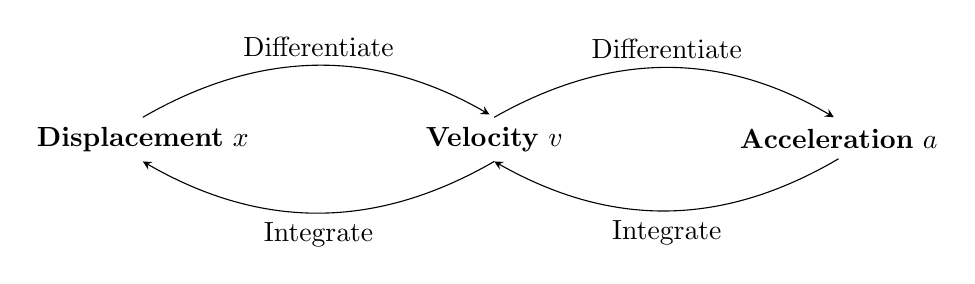
\begin{tikzpicture}
  \node (disp) {\textbf{Displacement} $x$};
  \node[right=2cm of disp] (vel) {\textbf{Velocity} $v$};
  \node[right=2cm of vel] (acc) {\textbf{Acceleration} $a$};
  \draw[-stealth,shorten >= 2pt] (disp.north) to[bend left] node[midway,above] {Differentiate} (vel.north);
  \draw[-stealth] (vel.south) to[bend left] node[midway,below] {Integrate} (disp.south);
  \draw[-stealth,shorten >= 2pt] (vel.north) to[bend left] node[midway,above] {Differentiate} (acc.north);
    \draw[-stealth] (acc.south) to[bend left] node[midway,below] {Integrate} (vel.south);
\end{tikzpicture}
\newpage
\begin{center}
\underline{\huge Kinematics Example - Problems with calculus}
\end{center}
\textit{A particle P moves along the x-axis in a straight line so that, at time t seconds, the velocity of P is $v \ \text{ms}^{-1}$, where}\\
\\
$
  v=\left\{
  \begin{array}{@{}ll@{}}
    10t-2t^2, & \text{for}\ 0\leqslant t \leqslant 6  \\
    -\dfrac{432}{t^2}, & t>6
  \end{array}\right.
$\\
\\
\\
\textit{At $t = 0$, P is at the origin O. Find the displacement of P from O when}\\
\\
$\mathit{t = 6}$\\
\\
\textbf{Integrate velocity}\\
\\
\textcolor{red}{$\mathlarger{x=\int v \ dt}$}\\
\\
$x=\int 10t-2t^2 \ dt= 5t^2-\frac{2}{3}t^3+c$\\
\\
\\
\textbf{Substitute in the value of t}\\
\\
$t=6$\\
\\
$x=5\times6^2-\frac{2}{3}\times6^3=36m$\\
\\
\\
$\mathit{t = 10}$
\\
\textbf{Integrate velocity for the second half of the journey}\\
\\
$x=\mathlarger{\int-\dfrac{432}{t^2} \ dt=\int-432t^{-2} \ dt=\dfrac{-432t^{-1}}{-1}+k=\dfrac{432}{t}+k}$\\
\\
\textbf{Find value of k by using known distance at t=6}\\
\\
$t=6 \ \ x=36$\\
\\
$36=\dfrac{432}{6}+k$\\
\\
$k=36-72=-36$\\
\\
\textbf{Find distance using value of k and t}\\
\\
$t=10$\\
\\
$x=\dfrac{432}{10}-36=7.2\text{m}$
\newpage
\begin{center}
\underline{\huge Kinematics Example - Finding direction of motion}
\end{center}
\textit{At $t=0$ a particle P is projected from a fixed point O with velocity $(7i+7\sqrt{3})ms^{-1}$. The particle moves freely under gravity. The position vector of a point on the path of P is $(x\mathbf{i}+y\mathbf{j})$m relative to O.}\\
\textit{Show that:}
$$y=\sqrt{3}x-\frac{g}{98}x^2$$
\\
\\
$x$ has constant velocity so write in terms of t
\begin{equation}\label{eq:1}
x=7t
\end{equation}
Write an equation for y using $s=ut+\frac{1}{2}at^2$
\begin{equation}\label{eq:2}
y=7\sqrt{3}t-\frac{g}{2}t^2
\end{equation}
Substitute \eqref{eq:1} into the \eqref{eq:2}
$$y=\sqrt{3}x-\frac{g}{2}\times\Big(\frac{x}{7}\Big)^2$$
Simplify
\begin{equation}\label{eq:3}
y=\sqrt{3}x-\frac{g}{98}x^2
\end{equation}
\\
\textit{Find the direction of motion of P when it passes through the point on the path where $x=20$}\\
\\
Differentiate \eqref{eq:3}
$$\frac{dy}{dx}=\sqrt{3}-\frac{2gx}{98}$$
Substitute in the value of x
$$\frac{dy}{dx}=\sqrt{3}-\frac{40g}{98}$$
\\
\textcolor{red}{Arctan(gradient)=Angle to the positive horizontal as $\dfrac{dy}{dx}$ is the same as $\dfrac{O}{A}$
}
\\
Perform arctan on the gradient to find the angle
$$\arctan\Big(\sqrt{3}-\frac{40g}{98}\Big)=-66.2$$
\newpage
\begin{center}
\underline{\Huge Problems with Vectors}
\end{center}
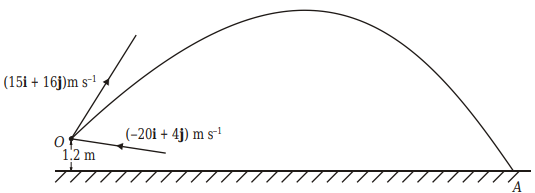
\includegraphics[width=10cm]{vector_problems.png}\\
\textit{A ball B of mass 0.4 kg is struck by a bat at a point O which is 1.2 m above horizontal ground.
The unit vectors i and j are respectively horizontal and vertical. Immediately before being
struck, B has velocity $(-20i+4j) \ ms^{–1}$. Immediately after being struck it has velocity $(15i+
16j) \ ms^{–1}$.\\
After B has been struck, it moves freely under gravity and strikes the ground at the point A, as
shown in the diagram above. The ball is modelled as a particle.}\\
\\
\textit{Calculate the magnitude of the impulse exerted by the bat on B. }
\textcolor{red}{$$I=m(v-u)$$}
Calculate the impulse as a vector using information from the question
$$I=0.4(15i+16j-(-20i+4j)=14i+4.8j$$
Calculate the magnitude of this vector
$$|I|=\sqrt{14^2+4.8^2}=14.5Ns$$
\\
\textit{By using the principle of conservation of energy, or otherwise, find the speed of B when
it reaches A.}
Initial energy:
$$\frac{1}{2}\times0.4\times\Big(\sqrt{15^2+16^2}\Big)^2=96.2J$$
Energy gained from loss in GPE
$$0.4\times9.8\times1.2=4.704J$$
Add energies and set equal to final kinetic energy
$$4.704+96.2=\frac{1}{2}\times0.4\times v^2$$
Find v
$$v=\sqrt{\frac{4.704+96.2}{0.5\times0.4}}=22.46$$
\\
\textit{Calculate the angle which the velocity of B makes with the ground when B reaches A.}\\
Using the knowledge that horizontal velocity is constant and the speed is known, use cos to find the angle
$$\arccos\Bigg(\frac{15}{22.5}\Bigg)=48\degree$$
\\
\textit{State two additional physical factors which could be taken into account in a refinement of
the model of the situation which would make it more realistic}
\begin{itemize}
\item Air resistance
\item Wind
\item Rotation of ball (ball is not a particle)
\end{itemize}




\end{document}